% Options for packages loaded elsewhere
\PassOptionsToPackage{unicode}{hyperref}
\PassOptionsToPackage{hyphens}{url}
\PassOptionsToPackage{dvipsnames,svgnames,x11names}{xcolor}
%
\documentclass[
  letterpaper,
  DIV=11,
  numbers=noendperiod]{scrartcl}

\usepackage{amsmath,amssymb}
\usepackage{iftex}
\ifPDFTeX
  \usepackage[T1]{fontenc}
  \usepackage[utf8]{inputenc}
  \usepackage{textcomp} % provide euro and other symbols
\else % if luatex or xetex
  \usepackage{unicode-math}
  \defaultfontfeatures{Scale=MatchLowercase}
  \defaultfontfeatures[\rmfamily]{Ligatures=TeX,Scale=1}
\fi
\usepackage{lmodern}
\ifPDFTeX\else  
    % xetex/luatex font selection
\fi
% Use upquote if available, for straight quotes in verbatim environments
\IfFileExists{upquote.sty}{\usepackage{upquote}}{}
\IfFileExists{microtype.sty}{% use microtype if available
  \usepackage[]{microtype}
  \UseMicrotypeSet[protrusion]{basicmath} % disable protrusion for tt fonts
}{}
\makeatletter
\@ifundefined{KOMAClassName}{% if non-KOMA class
  \IfFileExists{parskip.sty}{%
    \usepackage{parskip}
  }{% else
    \setlength{\parindent}{0pt}
    \setlength{\parskip}{6pt plus 2pt minus 1pt}}
}{% if KOMA class
  \KOMAoptions{parskip=half}}
\makeatother
\usepackage{xcolor}
\setlength{\emergencystretch}{3em} % prevent overfull lines
\setcounter{secnumdepth}{-\maxdimen} % remove section numbering
% Make \paragraph and \subparagraph free-standing
\ifx\paragraph\undefined\else
  \let\oldparagraph\paragraph
  \renewcommand{\paragraph}[1]{\oldparagraph{#1}\mbox{}}
\fi
\ifx\subparagraph\undefined\else
  \let\oldsubparagraph\subparagraph
  \renewcommand{\subparagraph}[1]{\oldsubparagraph{#1}\mbox{}}
\fi

\usepackage{color}
\usepackage{fancyvrb}
\newcommand{\VerbBar}{|}
\newcommand{\VERB}{\Verb[commandchars=\\\{\}]}
\DefineVerbatimEnvironment{Highlighting}{Verbatim}{commandchars=\\\{\}}
% Add ',fontsize=\small' for more characters per line
\usepackage{framed}
\definecolor{shadecolor}{RGB}{241,243,245}
\newenvironment{Shaded}{\begin{snugshade}}{\end{snugshade}}
\newcommand{\AlertTok}[1]{\textcolor[rgb]{0.68,0.00,0.00}{#1}}
\newcommand{\AnnotationTok}[1]{\textcolor[rgb]{0.37,0.37,0.37}{#1}}
\newcommand{\AttributeTok}[1]{\textcolor[rgb]{0.40,0.45,0.13}{#1}}
\newcommand{\BaseNTok}[1]{\textcolor[rgb]{0.68,0.00,0.00}{#1}}
\newcommand{\BuiltInTok}[1]{\textcolor[rgb]{0.00,0.23,0.31}{#1}}
\newcommand{\CharTok}[1]{\textcolor[rgb]{0.13,0.47,0.30}{#1}}
\newcommand{\CommentTok}[1]{\textcolor[rgb]{0.37,0.37,0.37}{#1}}
\newcommand{\CommentVarTok}[1]{\textcolor[rgb]{0.37,0.37,0.37}{\textit{#1}}}
\newcommand{\ConstantTok}[1]{\textcolor[rgb]{0.56,0.35,0.01}{#1}}
\newcommand{\ControlFlowTok}[1]{\textcolor[rgb]{0.00,0.23,0.31}{#1}}
\newcommand{\DataTypeTok}[1]{\textcolor[rgb]{0.68,0.00,0.00}{#1}}
\newcommand{\DecValTok}[1]{\textcolor[rgb]{0.68,0.00,0.00}{#1}}
\newcommand{\DocumentationTok}[1]{\textcolor[rgb]{0.37,0.37,0.37}{\textit{#1}}}
\newcommand{\ErrorTok}[1]{\textcolor[rgb]{0.68,0.00,0.00}{#1}}
\newcommand{\ExtensionTok}[1]{\textcolor[rgb]{0.00,0.23,0.31}{#1}}
\newcommand{\FloatTok}[1]{\textcolor[rgb]{0.68,0.00,0.00}{#1}}
\newcommand{\FunctionTok}[1]{\textcolor[rgb]{0.28,0.35,0.67}{#1}}
\newcommand{\ImportTok}[1]{\textcolor[rgb]{0.00,0.46,0.62}{#1}}
\newcommand{\InformationTok}[1]{\textcolor[rgb]{0.37,0.37,0.37}{#1}}
\newcommand{\KeywordTok}[1]{\textcolor[rgb]{0.00,0.23,0.31}{#1}}
\newcommand{\NormalTok}[1]{\textcolor[rgb]{0.00,0.23,0.31}{#1}}
\newcommand{\OperatorTok}[1]{\textcolor[rgb]{0.37,0.37,0.37}{#1}}
\newcommand{\OtherTok}[1]{\textcolor[rgb]{0.00,0.23,0.31}{#1}}
\newcommand{\PreprocessorTok}[1]{\textcolor[rgb]{0.68,0.00,0.00}{#1}}
\newcommand{\RegionMarkerTok}[1]{\textcolor[rgb]{0.00,0.23,0.31}{#1}}
\newcommand{\SpecialCharTok}[1]{\textcolor[rgb]{0.37,0.37,0.37}{#1}}
\newcommand{\SpecialStringTok}[1]{\textcolor[rgb]{0.13,0.47,0.30}{#1}}
\newcommand{\StringTok}[1]{\textcolor[rgb]{0.13,0.47,0.30}{#1}}
\newcommand{\VariableTok}[1]{\textcolor[rgb]{0.07,0.07,0.07}{#1}}
\newcommand{\VerbatimStringTok}[1]{\textcolor[rgb]{0.13,0.47,0.30}{#1}}
\newcommand{\WarningTok}[1]{\textcolor[rgb]{0.37,0.37,0.37}{\textit{#1}}}

\providecommand{\tightlist}{%
  \setlength{\itemsep}{0pt}\setlength{\parskip}{0pt}}\usepackage{longtable,booktabs,array}
\usepackage{calc} % for calculating minipage widths
% Correct order of tables after \paragraph or \subparagraph
\usepackage{etoolbox}
\makeatletter
\patchcmd\longtable{\par}{\if@noskipsec\mbox{}\fi\par}{}{}
\makeatother
% Allow footnotes in longtable head/foot
\IfFileExists{footnotehyper.sty}{\usepackage{footnotehyper}}{\usepackage{footnote}}
\makesavenoteenv{longtable}
\usepackage{graphicx}
\makeatletter
\def\maxwidth{\ifdim\Gin@nat@width>\linewidth\linewidth\else\Gin@nat@width\fi}
\def\maxheight{\ifdim\Gin@nat@height>\textheight\textheight\else\Gin@nat@height\fi}
\makeatother
% Scale images if necessary, so that they will not overflow the page
% margins by default, and it is still possible to overwrite the defaults
% using explicit options in \includegraphics[width, height, ...]{}
\setkeys{Gin}{width=\maxwidth,height=\maxheight,keepaspectratio}
% Set default figure placement to htbp
\makeatletter
\def\fps@figure{htbp}
\makeatother

\KOMAoption{captions}{tableheading}
\makeatletter
\makeatother
\makeatletter
\makeatother
\makeatletter
\@ifpackageloaded{caption}{}{\usepackage{caption}}
\AtBeginDocument{%
\ifdefined\contentsname
  \renewcommand*\contentsname{Table of contents}
\else
  \newcommand\contentsname{Table of contents}
\fi
\ifdefined\listfigurename
  \renewcommand*\listfigurename{List of Figures}
\else
  \newcommand\listfigurename{List of Figures}
\fi
\ifdefined\listtablename
  \renewcommand*\listtablename{List of Tables}
\else
  \newcommand\listtablename{List of Tables}
\fi
\ifdefined\figurename
  \renewcommand*\figurename{Figure}
\else
  \newcommand\figurename{Figure}
\fi
\ifdefined\tablename
  \renewcommand*\tablename{Table}
\else
  \newcommand\tablename{Table}
\fi
}
\@ifpackageloaded{float}{}{\usepackage{float}}
\floatstyle{ruled}
\@ifundefined{c@chapter}{\newfloat{codelisting}{h}{lop}}{\newfloat{codelisting}{h}{lop}[chapter]}
\floatname{codelisting}{Listing}
\newcommand*\listoflistings{\listof{codelisting}{List of Listings}}
\makeatother
\makeatletter
\@ifpackageloaded{caption}{}{\usepackage{caption}}
\@ifpackageloaded{subcaption}{}{\usepackage{subcaption}}
\makeatother
\makeatletter
\@ifpackageloaded{tcolorbox}{}{\usepackage[skins,breakable]{tcolorbox}}
\makeatother
\makeatletter
\@ifundefined{shadecolor}{\definecolor{shadecolor}{rgb}{.97, .97, .97}}
\makeatother
\makeatletter
\makeatother
\makeatletter
\makeatother
\ifLuaTeX
  \usepackage{selnolig}  % disable illegal ligatures
\fi
\IfFileExists{bookmark.sty}{\usepackage{bookmark}}{\usepackage{hyperref}}
\IfFileExists{xurl.sty}{\usepackage{xurl}}{} % add URL line breaks if available
\urlstyle{same} % disable monospaced font for URLs
\hypersetup{
  pdftitle={Data Analysis},
  pdfauthor={Kunal Khurana},
  colorlinks=true,
  linkcolor={blue},
  filecolor={Maroon},
  citecolor={Blue},
  urlcolor={Blue},
  pdfcreator={LaTeX via pandoc}}

\title{Data Analysis}
\usepackage{etoolbox}
\makeatletter
\providecommand{\subtitle}[1]{% add subtitle to \maketitle
  \apptocmd{\@title}{\par {\large #1 \par}}{}{}
}
\makeatother
\subtitle{basics}
\author{Kunal Khurana}
\date{2023-01-16}

\begin{document}
\maketitle
\ifdefined\Shaded\renewenvironment{Shaded}{\begin{tcolorbox}[breakable, boxrule=0pt, interior hidden, borderline west={3pt}{0pt}{shadecolor}, sharp corners, enhanced, frame hidden]}{\end{tcolorbox}}\fi

\renewcommand*\contentsname{Table of contents}
{
\hypersetup{linkcolor=}
\setcounter{tocdepth}{3}
\tableofcontents
}
\hypertarget{section}{%
\section{}\label{section}}

1. Introduction

In this exercies, we'll predict the probability of customer exiting the
bank or not with classification techniques.

\hypertarget{section-1}{%
\section{}\label{section-1}}

2. Dataset Overview

\hypertarget{section-2}{%
\subsection{}\label{section-2}}

2.1 Loading Libraries

\begin{Shaded}
\begin{Highlighting}[]
\CommentTok{\# import libraries}

\ImportTok{import}\NormalTok{ warnings }\ImportTok{as}\NormalTok{ wrn}
\NormalTok{wrn.filterwarnings(}\StringTok{\textquotesingle{}ignore\textquotesingle{}}\NormalTok{, category }\OperatorTok{=} \PreprocessorTok{DeprecationWarning}\NormalTok{) }
\NormalTok{wrn.filterwarnings(}\StringTok{\textquotesingle{}ignore\textquotesingle{}}\NormalTok{, category }\OperatorTok{=} \PreprocessorTok{FutureWarning}\NormalTok{) }
\NormalTok{wrn.filterwarnings(}\StringTok{\textquotesingle{}ignore\textquotesingle{}}\NormalTok{, category }\OperatorTok{=} \PreprocessorTok{UserWarning}\NormalTok{) }

\CommentTok{\#import optuna}
\CommentTok{\#import xgboost as xgb}
\ImportTok{import}\NormalTok{ pandas }\ImportTok{as}\NormalTok{ pd}
\ImportTok{import}\NormalTok{ matplotlib.pyplot }\ImportTok{as}\NormalTok{ plt}
\ImportTok{import}\NormalTok{ numpy }\ImportTok{as}\NormalTok{ np}
\ImportTok{import}\NormalTok{ scipy.stats }\ImportTok{as}\NormalTok{ stats}
\ImportTok{import}\NormalTok{ seaborn }\ImportTok{as}\NormalTok{ sns}
\ImportTok{import}\NormalTok{ matplotlib.pyplot }\ImportTok{as}\NormalTok{ plt}
\ImportTok{from}\NormalTok{ sklearn.model\_selection }\ImportTok{import}\NormalTok{ GroupKFold}
\ImportTok{from}\NormalTok{ sklearn.metrics }\ImportTok{import}\NormalTok{ accuracy\_score, classification\_report, mean\_absolute\_error}
\ImportTok{from}\NormalTok{ sklearn.ensemble }\ImportTok{import}\NormalTok{ RandomForestRegressor}
\ImportTok{from}\NormalTok{ sklearn.svm }\ImportTok{import}\NormalTok{ LinearSVC}
\ImportTok{from}\NormalTok{ sklearn.preprocessing }\ImportTok{import}\NormalTok{ RobustScaler}
\ImportTok{from}\NormalTok{ sklearn.pipeline }\ImportTok{import}\NormalTok{ make\_pipeline}
\ImportTok{from}\NormalTok{ sklearn.decomposition }\ImportTok{import}\NormalTok{ PCA}
\ImportTok{from}\NormalTok{ sklearn.model\_selection }\ImportTok{import}\NormalTok{ cross\_val\_score}
\ImportTok{from}\NormalTok{ sklearn.metrics }\ImportTok{import}\NormalTok{ make\_scorer, accuracy\_score, median\_absolute\_error}
\CommentTok{\#from imblearn.over\_sampling import RandomOverSampler}
\ImportTok{from}\NormalTok{ sklearn.model\_selection }\ImportTok{import}\NormalTok{ train\_test\_split}
\ImportTok{from}\NormalTok{ sklearn.preprocessing }\ImportTok{import}\NormalTok{ LabelEncoder}
\ImportTok{from}\NormalTok{ sklearn.metrics }\ImportTok{import}\NormalTok{ mean\_squared\_error, r2\_score}
\CommentTok{\#import lightgbm as lgb}
\ImportTok{import}\NormalTok{ numpy }\ImportTok{as}\NormalTok{ np}
\ImportTok{from}\NormalTok{ scipy }\ImportTok{import}\NormalTok{ stats}
\end{Highlighting}
\end{Shaded}

\begin{Shaded}
\begin{Highlighting}[]
\CommentTok{\# reading .csv files}

\NormalTok{train\_data }\OperatorTok{=}\NormalTok{ pd.read\_csv(}\StringTok{\textquotesingle{}train\_bank.csv\textquotesingle{}}\NormalTok{)}
\NormalTok{test\_data }\OperatorTok{=}\NormalTok{ pd.read\_csv(}\StringTok{\textquotesingle{}test.csv\textquotesingle{}}\NormalTok{)}
\NormalTok{orignal\_data }\OperatorTok{=}\NormalTok{ pd.read\_csv(}\StringTok{\textquotesingle{}Churn\_Modelling.csv\textquotesingle{}}\NormalTok{)}

\end{Highlighting}
\end{Shaded}

\hypertarget{section-3}{%
\subsection{}\label{section-3}}

2.2 Initial Observations and Trends

\begin{Shaded}
\begin{Highlighting}[]
\NormalTok{train\_data.head()}
\end{Highlighting}
\end{Shaded}

\begin{longtable}[]{@{}lllllllllllllll@{}}
\toprule\noalign{}
& id & CustomerId & Surname & CreditScore & Geography & Gender & Age &
Tenure & Balance & NumOfProducts & HasCrCard & IsActiveMember &
EstimatedSalary & Exited \\
\midrule\noalign{}
\endhead
\bottomrule\noalign{}
\endlastfoot
0 & 0 & 15674932 & Okwudilichukwu & 668 & France & Male & 33.0 & 3 &
0.00 & 2 & 1.0 & 0.0 & 181449.97 & 0 \\
1 & 1 & 15749177 & Okwudiliolisa & 627 & France & Male & 33.0 & 1 & 0.00
& 2 & 1.0 & 1.0 & 49503.50 & 0 \\
2 & 2 & 15694510 & Hsueh & 678 & France & Male & 40.0 & 10 & 0.00 & 2 &
1.0 & 0.0 & 184866.69 & 0 \\
3 & 3 & 15741417 & Kao & 581 & France & Male & 34.0 & 2 & 148882.54 & 1
& 1.0 & 1.0 & 84560.88 & 0 \\
4 & 4 & 15766172 & Chiemenam & 716 & Spain & Male & 33.0 & 5 & 0.00 & 2
& 1.0 & 1.0 & 15068.83 & 0 \\
\end{longtable}

\begin{Shaded}
\begin{Highlighting}[]
\NormalTok{test\_data.head()}
\end{Highlighting}
\end{Shaded}

\begin{longtable}[]{@{}llllllllllllll@{}}
\toprule\noalign{}
& id & CustomerId & Surname & CreditScore & Geography & Gender & Age &
Tenure & Balance & NumOfProducts & HasCrCard & IsActiveMember &
EstimatedSalary \\
\midrule\noalign{}
\endhead
\bottomrule\noalign{}
\endlastfoot
0 & 165034 & 15773898 & Lucchese & 586 & France & Female & 23.0 & 2 &
0.00 & 2 & 0.0 & 1.0 & 160976.75 \\
1 & 165035 & 15782418 & Nott & 683 & France & Female & 46.0 & 2 & 0.00 &
1 & 1.0 & 0.0 & 72549.27 \\
2 & 165036 & 15807120 & K? & 656 & France & Female & 34.0 & 7 & 0.00 & 2
& 1.0 & 0.0 & 138882.09 \\
3 & 165037 & 15808905 & O\textquotesingle Donnell & 681 & France & Male
& 36.0 & 8 & 0.00 & 1 & 1.0 & 0.0 & 113931.57 \\
4 & 165038 & 15607314 & Higgins & 752 & Germany & Male & 38.0 & 10 &
121263.62 & 1 & 1.0 & 0.0 & 139431.00 \\
\end{longtable}

\begin{Shaded}
\begin{Highlighting}[]
\NormalTok{orignal\_data.head()}
\end{Highlighting}
\end{Shaded}

\begin{longtable}[]{@{}lllllllllllllll@{}}
\toprule\noalign{}
& RowNumber & CustomerId & Surname & CreditScore & Geography & Gender &
Age & Tenure & Balance & NumOfProducts & HasCrCard & IsActiveMember &
EstimatedSalary & Exited \\
\midrule\noalign{}
\endhead
\bottomrule\noalign{}
\endlastfoot
0 & 1 & 15634602 & Hargrave & 619 & France & Female & 42.0 & 2 & 0.00 &
1 & 1.0 & 1.0 & 101348.88 & 1 \\
1 & 2 & 15647311 & Hill & 608 & Spain & Female & 41.0 & 1 & 83807.86 & 1
& 0.0 & 1.0 & 112542.58 & 0 \\
2 & 3 & 15619304 & Onio & 502 & France & Female & 42.0 & 8 & 159660.80 &
3 & 1.0 & 0.0 & 113931.57 & 1 \\
3 & 4 & 15701354 & Boni & 699 & France & Female & 39.0 & 1 & 0.00 & 2 &
0.0 & 0.0 & 93826.63 & 0 \\
4 & 5 & 15737888 & Mitchell & 850 & Spain & Female & 43.0 & 2 &
125510.82 & 1 & NaN & 1.0 & 79084.10 & 0 \\
\end{longtable}

\begin{Shaded}
\begin{Highlighting}[]
\CommentTok{\# checking the number of rows and columns}

\NormalTok{num\_train\_rows, num\_train\_columns }\OperatorTok{=}\NormalTok{ train\_data.shape}

\NormalTok{num\_test\_rows, num\_test\_columns }\OperatorTok{=}\NormalTok{ test\_data.shape}

\NormalTok{num\_orignal\_rows, num\_orignal\_columns }\OperatorTok{=}\NormalTok{ orignal\_data.shape}

\BuiltInTok{print}\NormalTok{(}\StringTok{\textquotesingle{}Training Data: \textquotesingle{}}\NormalTok{)}
\BuiltInTok{print}\NormalTok{(}\SpecialStringTok{f"Number of Rows: }\SpecialCharTok{\{}\NormalTok{num\_train\_rows}\SpecialCharTok{\}}\SpecialStringTok{"}\NormalTok{)}
\BuiltInTok{print}\NormalTok{(}\SpecialStringTok{f"Number of Columns: }\SpecialCharTok{\{}\NormalTok{num\_train\_columns}\SpecialCharTok{\}}\CharTok{\textbackslash{}n}\SpecialStringTok{"}\NormalTok{)}

\BuiltInTok{print}\NormalTok{(}\StringTok{\textquotesingle{}Test Data: \textquotesingle{}}\NormalTok{)}
\BuiltInTok{print}\NormalTok{(}\SpecialStringTok{f"Number of Rows: }\SpecialCharTok{\{}\NormalTok{num\_test\_rows}\SpecialCharTok{\}}\SpecialStringTok{"}\NormalTok{)}
\BuiltInTok{print}\NormalTok{(}\SpecialStringTok{f"Number of Columns :}\SpecialCharTok{\{}\NormalTok{num\_test\_columns}\SpecialCharTok{\}}\CharTok{\textbackslash{}n}\SpecialStringTok{"}\NormalTok{)}

\BuiltInTok{print}\NormalTok{(}\StringTok{"Orignal Data: "}\NormalTok{)}
\BuiltInTok{print}\NormalTok{(}\SpecialStringTok{f"Number of Rows: }\SpecialCharTok{\{}\NormalTok{num\_orignal\_rows}\SpecialCharTok{\}}\SpecialStringTok{"}\NormalTok{)}
\BuiltInTok{print}\NormalTok{(}\SpecialStringTok{f"Number of Columns: }\SpecialCharTok{\{}\NormalTok{num\_orignal\_columns}\SpecialCharTok{\}}\SpecialStringTok{"}\NormalTok{)}

\end{Highlighting}
\end{Shaded}

\begin{verbatim}
Training Data: 
Number of Rows: 165034
Number of Columns: 14

Test Data: 
Number of Rows: 110023
Number of Columns :13

Orignal Data: 
Number of Rows: 10002
Number of Columns: 14
\end{verbatim}

\begin{Shaded}
\begin{Highlighting}[]
\CommentTok{\# create a table for missing values, unique values, and data types}

\NormalTok{missing\_values\_train }\OperatorTok{=}\NormalTok{ pd.DataFrame(\{}
    \StringTok{\textquotesingle{}Feature\textquotesingle{}}\NormalTok{: train\_data.columns,}
    \StringTok{\textquotesingle{}[TRAIN] No. of Missing Values\textquotesingle{}}\NormalTok{ : train\_data.isnull().}\BuiltInTok{sum}\NormalTok{().values,}
    \StringTok{\textquotesingle{}[TRAIN] }\SpecialCharTok{\% o}\StringTok{f Missing Values\textquotesingle{}}\NormalTok{ : ((train\_data.isnull().}\BuiltInTok{sum}\NormalTok{().values)}\OperatorTok{/}\BuiltInTok{len}\NormalTok{(train\_data)}\OperatorTok{*}\DecValTok{100}\NormalTok{)}
\NormalTok{\})}

\NormalTok{missing\_values\_test }\OperatorTok{=}\NormalTok{ pd.DataFrame(\{}
    \StringTok{\textquotesingle{}Feature\textquotesingle{}}\NormalTok{ : test\_data.columns,}
    \StringTok{\textquotesingle{}[TEST] No. of Missing Values\textquotesingle{}}\NormalTok{ : test\_data.isnull().}\BuiltInTok{sum}\NormalTok{().values,}
    \StringTok{\textquotesingle{}[TEST]}\SpecialCharTok{\% o}\StringTok{f Missing Values\textquotesingle{}}\NormalTok{: ((test\_data.isnull().}\BuiltInTok{sum}\NormalTok{().values)}\OperatorTok{/}\BuiltInTok{len}\NormalTok{(test\_data)}\OperatorTok{*}\DecValTok{100}\NormalTok{)}
\NormalTok{\})}
                                    
\NormalTok{missing\_values\_orignal }\OperatorTok{=}\NormalTok{ pd.DataFrame(\{}
    \StringTok{\textquotesingle{}Feature\textquotesingle{}}\NormalTok{ : orignal\_data.columns,}
    \StringTok{\textquotesingle{}[ORIGNAL] No. of Missing Values\textquotesingle{}}\NormalTok{: orignal\_data.isnull().}\BuiltInTok{sum}\NormalTok{().values,}
    \StringTok{\textquotesingle{}[ORIGNAL] }\SpecialCharTok{\% o}\StringTok{f Missing Values\textquotesingle{}}\NormalTok{ : ((orignal\_data.isnull().}\BuiltInTok{sum}\NormalTok{().values)}\OperatorTok{/}\BuiltInTok{len}\NormalTok{(orignal\_data)}\OperatorTok{*}\DecValTok{100}\NormalTok{)}
\NormalTok{\})}
\end{Highlighting}
\end{Shaded}

\begin{Shaded}
\begin{Highlighting}[]
\NormalTok{unique\_values }\OperatorTok{=}\NormalTok{ pd.DataFrame(\{}
    \StringTok{\textquotesingle{}Feature\textquotesingle{}}\NormalTok{: train\_data.columns,}
    \StringTok{\textquotesingle{}No. of Unique Values [FROM TRAIN]\textquotesingle{}}\NormalTok{ :train\_data.nunique().values}
\NormalTok{\})}

\NormalTok{feature\_types }\OperatorTok{=}\NormalTok{ pd.DataFrame(\{}
    \StringTok{\textquotesingle{}Feature\textquotesingle{}}\NormalTok{: train\_data.columns,}
    \StringTok{\textquotesingle{}DataType\textquotesingle{}}\NormalTok{: train\_data.dtypes}
\NormalTok{\})}
\end{Highlighting}
\end{Shaded}

\begin{Shaded}
\begin{Highlighting}[]
\NormalTok{merged\_df }\OperatorTok{=}\NormalTok{ pd.merge(missing\_values\_train, missing\_values\_test, on}\OperatorTok{=} \StringTok{\textquotesingle{}Feature\textquotesingle{}}\NormalTok{, how}\OperatorTok{=} \StringTok{\textquotesingle{}left\textquotesingle{}}\NormalTok{)}
\NormalTok{merged\_df }\OperatorTok{=}\NormalTok{ pd.merge(merged\_df, missing\_values\_orignal, on }\OperatorTok{=} \StringTok{\textquotesingle{}Feature\textquotesingle{}}\NormalTok{, how }\OperatorTok{=} \StringTok{\textquotesingle{}left\textquotesingle{}}\NormalTok{)}
\NormalTok{merged\_df }\OperatorTok{=}\NormalTok{ pd.merge(merged\_df, unique\_values, on}\OperatorTok{=} \StringTok{\textquotesingle{}Feature\textquotesingle{}}\NormalTok{, how}\OperatorTok{=} \StringTok{\textquotesingle{}left\textquotesingle{}}\NormalTok{)}
\NormalTok{merged\_df }\OperatorTok{=}\NormalTok{ pd.merge(merged\_df, feature\_types, on }\OperatorTok{=} \StringTok{\textquotesingle{}Feature\textquotesingle{}}\NormalTok{, how}\OperatorTok{=} \StringTok{\textquotesingle{}left\textquotesingle{}}\NormalTok{)}

\NormalTok{merged\_df}
\end{Highlighting}
\end{Shaded}

\begin{longtable}[]{@{}llllllllll@{}}
\toprule\noalign{}
& Feature & {[}TRAIN{]} No. of Missing Values & {[}TRAIN{]} \% of
Missing Values & {[}TEST{]} No. of Missing Values & {[}TEST{]}\% of
Missing Values & {[}ORIGNAL{]} No. of Missing Values & {[}ORIGNAL{]} \%
of Missing Values & No. of Unique Values {[}FROM TRAIN{]} & DataType \\
\midrule\noalign{}
\endhead
\bottomrule\noalign{}
\endlastfoot
0 & id & 0 & 0.0 & 0.0 & 0.0 & NaN & NaN & 165034 & int64 \\
1 & CustomerId & 0 & 0.0 & 0.0 & 0.0 & 0.0 & 0.000000 & 23221 & int64 \\
2 & Surname & 0 & 0.0 & 0.0 & 0.0 & 0.0 & 0.000000 & 2797 & object \\
3 & CreditScore & 0 & 0.0 & 0.0 & 0.0 & 0.0 & 0.000000 & 457 & int64 \\
4 & Geography & 0 & 0.0 & 0.0 & 0.0 & 1.0 & 0.009998 & 3 & object \\
5 & Gender & 0 & 0.0 & 0.0 & 0.0 & 0.0 & 0.000000 & 2 & object \\
6 & Age & 0 & 0.0 & 0.0 & 0.0 & 1.0 & 0.009998 & 71 & float64 \\
7 & Tenure & 0 & 0.0 & 0.0 & 0.0 & 0.0 & 0.000000 & 11 & int64 \\
8 & Balance & 0 & 0.0 & 0.0 & 0.0 & 0.0 & 0.000000 & 30075 & float64 \\
9 & NumOfProducts & 0 & 0.0 & 0.0 & 0.0 & 0.0 & 0.000000 & 4 & int64 \\
10 & HasCrCard & 0 & 0.0 & 0.0 & 0.0 & 1.0 & 0.009998 & 2 & float64 \\
11 & IsActiveMember & 0 & 0.0 & 0.0 & 0.0 & 1.0 & 0.009998 & 2 &
float64 \\
12 & EstimatedSalary & 0 & 0.0 & 0.0 & 0.0 & 0.0 & 0.000000 & 55298 &
float64 \\
13 & Exited & 0 & 0.0 & NaN & NaN & 0.0 & 0.000000 & 2 & int64 \\
\end{longtable}

\begin{Shaded}
\begin{Highlighting}[]
\CommentTok{\# count duplicate rows in train\_data}
\NormalTok{train\_duplicates }\OperatorTok{=}\NormalTok{ train\_data.duplicated().}\BuiltInTok{sum}\NormalTok{()}

\CommentTok{\# count duplicate rows in test\_data}
\NormalTok{test\_duplicates }\OperatorTok{=}\NormalTok{ test\_data.duplicated().}\BuiltInTok{sum}\NormalTok{()}

\CommentTok{\# count duplicate rows in orignal\_data}
\NormalTok{orignal\_duplicates }\OperatorTok{=}\NormalTok{ orignal\_data.duplicated().}\BuiltInTok{sum}\NormalTok{()}

\CommentTok{\# print results}
\BuiltInTok{print}\NormalTok{(}\SpecialStringTok{f"Number of duplicate rows in train\_data: }\SpecialCharTok{\{}\NormalTok{train\_duplicates}\SpecialCharTok{\}}\SpecialStringTok{"}\NormalTok{)}
\BuiltInTok{print}\NormalTok{(}\SpecialStringTok{f"Number of duplicate rows in test\_data: }\SpecialCharTok{\{}\NormalTok{test\_duplicates}\SpecialCharTok{\}}\SpecialStringTok{"}\NormalTok{)}
\BuiltInTok{print}\NormalTok{(}\SpecialStringTok{f"Number of duplicate rows in orignal\_data: }\SpecialCharTok{\{}\NormalTok{orignal\_duplicates}\SpecialCharTok{\}}\SpecialStringTok{"}\NormalTok{)}
\end{Highlighting}
\end{Shaded}

\begin{verbatim}
Number of duplicate rows in train_data: 0
Number of duplicate rows in test_data: 0
Number of duplicate rows in orignal_data: 2
\end{verbatim}

\begin{Shaded}
\begin{Highlighting}[]
\CommentTok{\# description of all numerical columns in the dataset}
\NormalTok{train\_data.describe().T}
\CommentTok{\#test\_data.describe().T}
\CommentTok{\#orignal\_data.describe().T}
\end{Highlighting}
\end{Shaded}

\begin{longtable}[]{@{}lllllllll@{}}
\toprule\noalign{}
& count & mean & std & min & 25\% & 50\% & 75\% & max \\
\midrule\noalign{}
\endhead
\bottomrule\noalign{}
\endlastfoot
id & 165034.0 & 8.251650e+04 & 47641.356500 & 0.00 & 41258.25 & 82516.5
& 1.237748e+05 & 165033.00 \\
CustomerId & 165034.0 & 1.569201e+07 & 71397.816791 & 15565701.00 &
15633141.00 & 15690169.0 & 1.575682e+07 & 15815690.00 \\
CreditScore & 165034.0 & 6.564544e+02 & 80.103340 & 350.00 & 597.00 &
659.0 & 7.100000e+02 & 850.00 \\
Age & 165034.0 & 3.812589e+01 & 8.867205 & 18.00 & 32.00 & 37.0 &
4.200000e+01 & 92.00 \\
Tenure & 165034.0 & 5.020353e+00 & 2.806159 & 0.00 & 3.00 & 5.0 &
7.000000e+00 & 10.00 \\
Balance & 165034.0 & 5.547809e+04 & 62817.663278 & 0.00 & 0.00 & 0.0 &
1.199395e+05 & 250898.09 \\
NumOfProducts & 165034.0 & 1.554455e+00 & 0.547154 & 1.00 & 1.00 & 2.0 &
2.000000e+00 & 4.00 \\
HasCrCard & 165034.0 & 7.539537e-01 & 0.430707 & 0.00 & 1.00 & 1.0 &
1.000000e+00 & 1.00 \\
IsActiveMember & 165034.0 & 4.977702e-01 & 0.499997 & 0.00 & 0.00 & 0.0
& 1.000000e+00 & 1.00 \\
EstimatedSalary & 165034.0 & 1.125748e+05 & 50292.865585 & 11.58 &
74637.57 & 117948.0 & 1.551525e+05 & 199992.48 \\
Exited & 165034.0 & 2.115988e-01 & 0.408443 & 0.00 & 0.00 & 0.0 &
0.000000e+00 & 1.00 \\
\end{longtable}

\hypertarget{section-4}{%
\section{}\label{section-4}}

3. EDA

\begin{Shaded}
\begin{Highlighting}[]
\NormalTok{numerical\_variables }\OperatorTok{=}\NormalTok{ [}\StringTok{\textquotesingle{}CreditScore\textquotesingle{}}\NormalTok{, }\StringTok{\textquotesingle{}Age\textquotesingle{}}\NormalTok{, }\StringTok{\textquotesingle{}Balance\textquotesingle{}}\NormalTok{, }\StringTok{\textquotesingle{}EstimatedSalary\textquotesingle{}}\NormalTok{]}
\NormalTok{target\_variable }\OperatorTok{=} \StringTok{\textquotesingle{}Exited\textquotesingle{}}
\NormalTok{categorical\_variables }\OperatorTok{=}\NormalTok{ [}\StringTok{\textquotesingle{}Geography\textquotesingle{}}\NormalTok{, }\StringTok{\textquotesingle{}Gender\textquotesingle{}}\NormalTok{, }\StringTok{\textquotesingle{}Tenure\textquotesingle{}}\NormalTok{, }\StringTok{\textquotesingle{}NumOfProducts\textquotesingle{}}\NormalTok{, }\StringTok{\textquotesingle{}HasCrCard\textquotesingle{}}\NormalTok{, }\StringTok{\textquotesingle{}IsActiveMember\textquotesingle{}}\NormalTok{]}
\end{Highlighting}
\end{Shaded}

\hypertarget{section-5}{%
\subsection{}\label{section-5}}

3.1 Numerical Features

\begin{Shaded}
\begin{Highlighting}[]
\CommentTok{\# Analysis}

\CommentTok{\# custom color pallete define}
\NormalTok{custom\_palette }\OperatorTok{=}\NormalTok{ [}\StringTok{\textquotesingle{}\#3498db\textquotesingle{}}\NormalTok{, }\StringTok{\textquotesingle{}\#e74c3c\textquotesingle{}}\NormalTok{,}\StringTok{\textquotesingle{}\#2ecc71\textquotesingle{}}\NormalTok{]}

\CommentTok{\# add \textquotesingle{}Dataset\textquotesingle{} column to distinguish between train and test data}
\NormalTok{train\_data[}\StringTok{\textquotesingle{}Dataset\textquotesingle{}}\NormalTok{] }\OperatorTok{=} \StringTok{\textquotesingle{}Train\textquotesingle{}}
\NormalTok{test\_data[}\StringTok{\textquotesingle{}Dataset\textquotesingle{}}\NormalTok{] }\OperatorTok{=} \StringTok{\textquotesingle{}Test\textquotesingle{}}
\NormalTok{orignal\_data[}\StringTok{\textquotesingle{}Dataset\textquotesingle{}}\NormalTok{]}\OperatorTok{=} \StringTok{\textquotesingle{}Orignal\textquotesingle{}}

\NormalTok{variables }\OperatorTok{=}\NormalTok{ [col }\ControlFlowTok{for}\NormalTok{ col }\KeywordTok{in}\NormalTok{ train\_data.columns }\ControlFlowTok{if}\NormalTok{ col }\KeywordTok{in}\NormalTok{ numerical\_variables]}

\CommentTok{\# function to create and display a row of plots for a single variable}
\KeywordTok{def}\NormalTok{ create\_variable\_plots(variable):}
\NormalTok{    sns.set\_style(}\StringTok{\textquotesingle{}whitegrid\textquotesingle{}}\NormalTok{)}
    
\NormalTok{    fig, axes }\OperatorTok{=}\NormalTok{ plt.subplots(}\DecValTok{1}\NormalTok{,}\DecValTok{2}\NormalTok{, figsize}\OperatorTok{=}\NormalTok{ (}\DecValTok{12}\NormalTok{, }\DecValTok{4}\NormalTok{))}
    
    \CommentTok{\#Box plot}
\NormalTok{    plt.subplot(}\DecValTok{1}\NormalTok{, }\DecValTok{2}\NormalTok{, }\DecValTok{1}\NormalTok{)}
\NormalTok{    sns.boxplot(data }\OperatorTok{=}\NormalTok{ pd.concat([}
\NormalTok{        train\_data, test\_data, orignal\_data.dropna()}
\NormalTok{    ]), }
\NormalTok{    x}\OperatorTok{=}\NormalTok{ variable, y }\OperatorTok{=} \StringTok{"Dataset"}\NormalTok{, palette}\OperatorTok{=}\NormalTok{ custom\_palette)}
\NormalTok{    plt.xlabel(variable)}
\NormalTok{    plt.title(}\SpecialStringTok{f"Box Plot for }\SpecialCharTok{\{}\NormalTok{variable}\SpecialCharTok{\}}\SpecialStringTok{"}\NormalTok{)}
    
    \CommentTok{\# Seperate Histograms}
\NormalTok{    plt.subplot(}\DecValTok{1}\NormalTok{,}\DecValTok{2}\NormalTok{,}\DecValTok{2}\NormalTok{)}
\NormalTok{    sns.histplot(data }\OperatorTok{=}\NormalTok{ train\_data, x }\OperatorTok{=}\NormalTok{ variable, color}\OperatorTok{=}\NormalTok{ custom\_palette[}\DecValTok{0}\NormalTok{], kde}\OperatorTok{=} \VariableTok{True}\NormalTok{, bins}\OperatorTok{=} \DecValTok{30}\NormalTok{, label}\OperatorTok{=} \StringTok{\textquotesingle{}Train\textquotesingle{}}\NormalTok{)}
\NormalTok{    sns.histplot(data }\OperatorTok{=}\NormalTok{ test\_data, x}\OperatorTok{=}\NormalTok{ variable, color}\OperatorTok{=}\NormalTok{ custom\_palette[}\DecValTok{1}\NormalTok{], kde}\OperatorTok{=} \VariableTok{True}\NormalTok{, bins}\OperatorTok{=} \DecValTok{30}\NormalTok{, label}\OperatorTok{=} \StringTok{\textquotesingle{}Test\textquotesingle{}}\NormalTok{)}
\NormalTok{    sns.histplot(data }\OperatorTok{=}\NormalTok{ orignal\_data.dropna(), x}\OperatorTok{=}\NormalTok{variable, color}\OperatorTok{=}\NormalTok{custom\_palette[}\DecValTok{2}\NormalTok{], kde}\OperatorTok{=}\VariableTok{True}\NormalTok{, bins}\OperatorTok{=}\DecValTok{30}\NormalTok{, label}\OperatorTok{=}\StringTok{"Original"}\NormalTok{)}
\NormalTok{    plt.xlabel(variable)}
\NormalTok{    plt.ylabel(}\StringTok{\textquotesingle{}Frequency\textquotesingle{}}\NormalTok{)}
\NormalTok{    plt.title(}\SpecialStringTok{f\textquotesingle{}Histogram for }\SpecialCharTok{\{}\NormalTok{variable}\SpecialCharTok{\}}\SpecialStringTok{ [TRAIN, TEST and ORIGNAL]\textquotesingle{}}\NormalTok{)}
\NormalTok{    plt.legend()}
    
    \CommentTok{\#adjust spacing between subplots}
\NormalTok{    plt.tight\_layout()}
    
    \CommentTok{\# show the plots}
\NormalTok{    plt.show()}

\CommentTok{\# perform univariate analysis for each variable}
\ControlFlowTok{for}\NormalTok{ variable }\KeywordTok{in}\NormalTok{ variables:}
\NormalTok{    create\_variable\_plots(variable)}
    
\CommentTok{\# drop the \textquotesingle{}Dataset\textquotesingle{} column after analysis}
\NormalTok{train\_data.drop(}\StringTok{\textquotesingle{}Dataset\textquotesingle{}}\NormalTok{, axis}\OperatorTok{=}\DecValTok{1}\NormalTok{, inplace }\OperatorTok{=} \VariableTok{True}\NormalTok{)}
\NormalTok{test\_data.drop(}\StringTok{\textquotesingle{}Dataset\textquotesingle{}}\NormalTok{, axis}\OperatorTok{=}\DecValTok{1}\NormalTok{, inplace}\OperatorTok{=} \VariableTok{True}\NormalTok{)}
\NormalTok{orignal\_data.drop(}\StringTok{\textquotesingle{}Dataset\textquotesingle{}}\NormalTok{, axis}\OperatorTok{=}\DecValTok{1}\NormalTok{, inplace}\OperatorTok{=}\VariableTok{True}\NormalTok{)}
\end{Highlighting}
\end{Shaded}

\begin{figure}[H]

{\centering 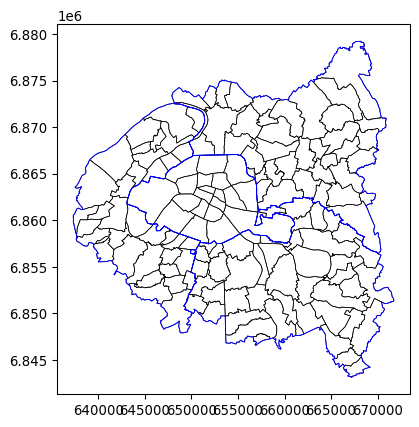
\includegraphics{EDA_Classification_files/figure-pdf/cell-14-output-1.png}

}

\end{figure}

\begin{figure}[H]

{\centering 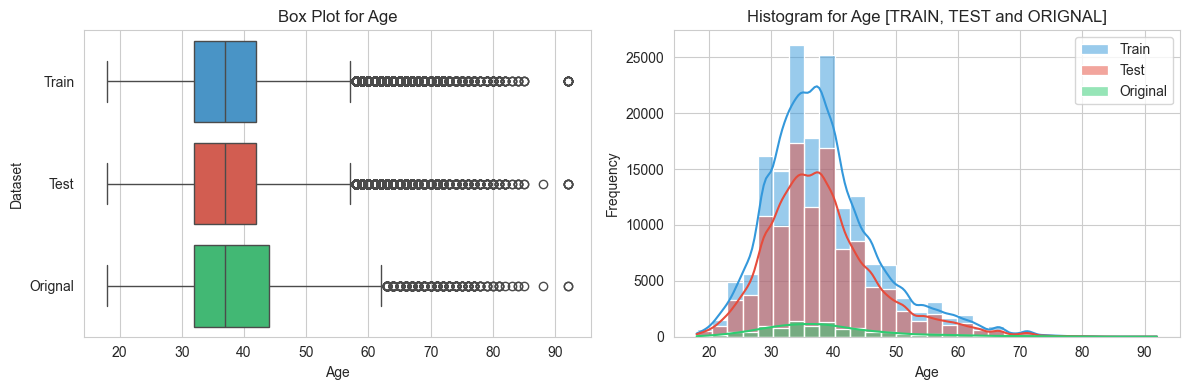
\includegraphics{EDA_Classification_files/figure-pdf/cell-14-output-2.png}

}

\end{figure}

\begin{figure}[H]

{\centering 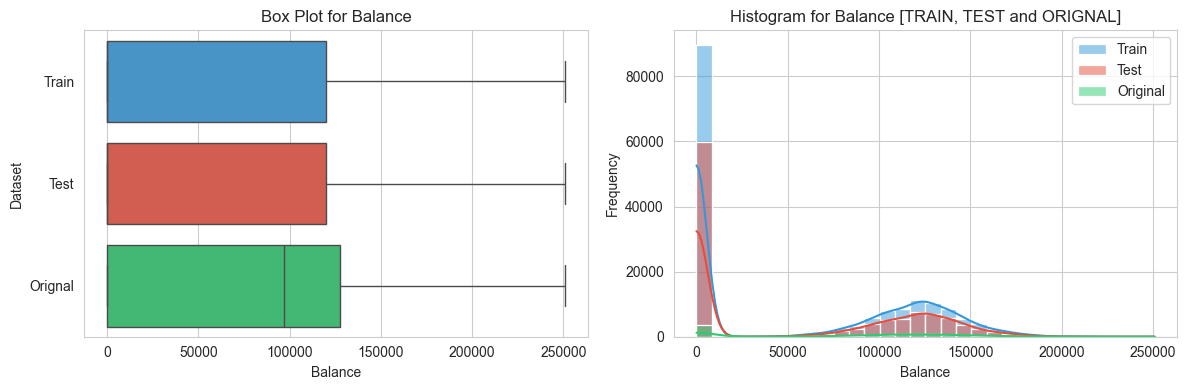
\includegraphics{EDA_Classification_files/figure-pdf/cell-14-output-3.png}

}

\end{figure}

\begin{figure}[H]

{\centering 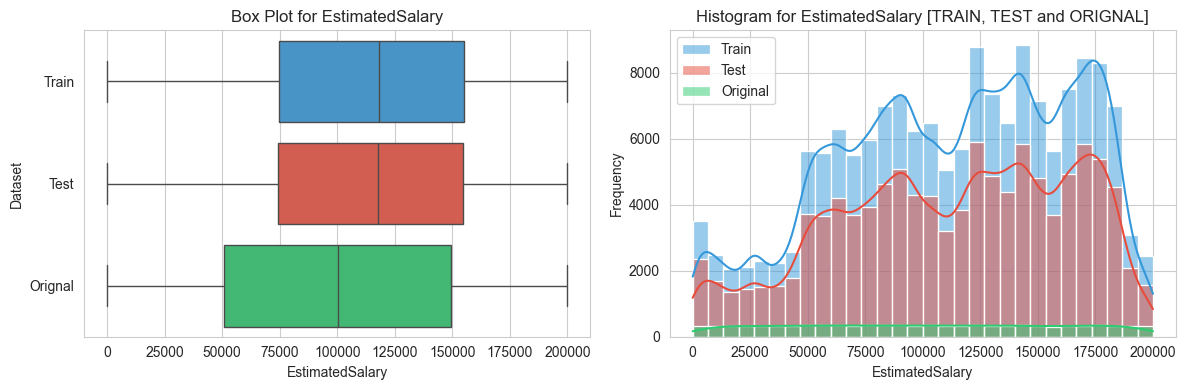
\includegraphics{EDA_Classification_files/figure-pdf/cell-14-output-4.png}

}

\end{figure}

\hypertarget{section-6}{%
\subsection{}\label{section-6}}

2

3.2 Categorical features

\begin{Shaded}
\begin{Highlighting}[]
\CommentTok{\# Analysis of all CATEGORICAL features}

\CommentTok{\# Define a custom color palette for categorical features}
\NormalTok{categorical\_palette }\OperatorTok{=}\NormalTok{ [}\StringTok{\textquotesingle{}\#3498db\textquotesingle{}}\NormalTok{, }\StringTok{\textquotesingle{}\#e74c3c\textquotesingle{}}\NormalTok{, }\StringTok{\textquotesingle{}\#2ecc71\textquotesingle{}}\NormalTok{, }\StringTok{\textquotesingle{}\#f39c12\textquotesingle{}}\NormalTok{, }\StringTok{\textquotesingle{}\#9b59b6\textquotesingle{}}\NormalTok{, }\StringTok{\textquotesingle{}\#bdc3c7\textquotesingle{}}\NormalTok{, }\StringTok{\textquotesingle{}\#1abc9c\textquotesingle{}}\NormalTok{, }\StringTok{\textquotesingle{}\#f1c40f\textquotesingle{}}\NormalTok{, }\StringTok{\textquotesingle{}\#95a5a6\textquotesingle{}}\NormalTok{, }\StringTok{\textquotesingle{}\#d35400\textquotesingle{}}\NormalTok{]}

\CommentTok{\# List of categorical variables}
\NormalTok{categorical\_variables }\OperatorTok{=}\NormalTok{ [col }\ControlFlowTok{for}\NormalTok{ col }\KeywordTok{in}\NormalTok{ categorical\_variables]}

\CommentTok{\# Function to create and display a row of plots for a single categorical variable}
\KeywordTok{def}\NormalTok{ create\_categorical\_plots(variable):}
\NormalTok{    sns.set\_style(}\StringTok{\textquotesingle{}whitegrid\textquotesingle{}}\NormalTok{)}
    
\NormalTok{    fig, axes }\OperatorTok{=}\NormalTok{ plt.subplots(}\DecValTok{1}\NormalTok{, }\DecValTok{2}\NormalTok{, figsize}\OperatorTok{=}\NormalTok{(}\DecValTok{12}\NormalTok{, }\DecValTok{4}\NormalTok{))}

    \CommentTok{\# Pie Chart}
\NormalTok{    plt.subplot(}\DecValTok{1}\NormalTok{, }\DecValTok{2}\NormalTok{, }\DecValTok{1}\NormalTok{)}
\NormalTok{    train\_data[variable].value\_counts().plot.pie(autopct}\OperatorTok{=}\StringTok{\textquotesingle{}}\SpecialCharTok{\%1.1f\%\%}\StringTok{\textquotesingle{}}\NormalTok{,}
\NormalTok{                                                 colors}\OperatorTok{=}\NormalTok{categorical\_palette, }
\NormalTok{                                                 wedgeprops}\OperatorTok{=}\BuiltInTok{dict}\NormalTok{(width}\OperatorTok{=}\FloatTok{0.3}\NormalTok{), }
\NormalTok{                                                 startangle}\OperatorTok{=}\DecValTok{140}\NormalTok{)}
\NormalTok{    plt.title(}\SpecialStringTok{f"Pie Chart for }\SpecialCharTok{\{}\NormalTok{variable}\SpecialCharTok{\}}\SpecialStringTok{"}\NormalTok{)}

    \CommentTok{\# Bar Graph}
\NormalTok{    plt.subplot(}\DecValTok{1}\NormalTok{, }\DecValTok{2}\NormalTok{, }\DecValTok{2}\NormalTok{)}
\NormalTok{    sns.countplot(data}\OperatorTok{=}\NormalTok{pd.concat([}
\NormalTok{        train\_data, test\_data, orignal\_data.dropna()}
\NormalTok{    ]), x}\OperatorTok{=}\NormalTok{variable, palette}\OperatorTok{=}\NormalTok{categorical\_palette)}
\NormalTok{    plt.xlabel(variable)}
\NormalTok{    plt.ylabel(}\StringTok{"Count"}\NormalTok{)}
\NormalTok{    plt.title(}\SpecialStringTok{f"Bar Graph for }\SpecialCharTok{\{}\NormalTok{variable}\SpecialCharTok{\}}\SpecialStringTok{ [TRAIN, TEST \& ORIGINAL]"}\NormalTok{)}

    \CommentTok{\# Adjust spacing between subplots}
\NormalTok{    plt.tight\_layout()}

    \CommentTok{\# Show the plots}
\NormalTok{    plt.show()}

\CommentTok{\# Perform univariate analysis for each categorical variable}
\ControlFlowTok{for}\NormalTok{ variable }\KeywordTok{in}\NormalTok{ categorical\_variables:}
\NormalTok{    create\_categorical\_plots(variable)}
\end{Highlighting}
\end{Shaded}

\begin{figure}[H]

{\centering 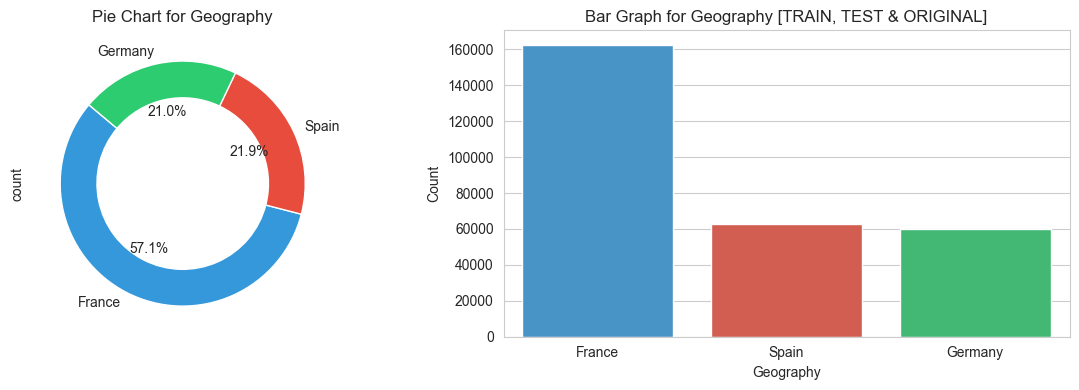
\includegraphics{EDA_Classification_files/figure-pdf/cell-15-output-1.png}

}

\end{figure}

\begin{figure}[H]

{\centering 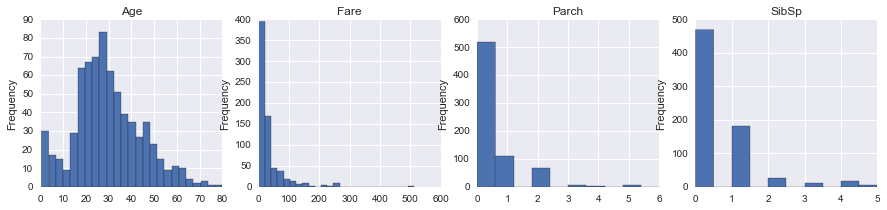
\includegraphics{EDA_Classification_files/figure-pdf/cell-15-output-2.png}

}

\end{figure}

\begin{figure}[H]

{\centering 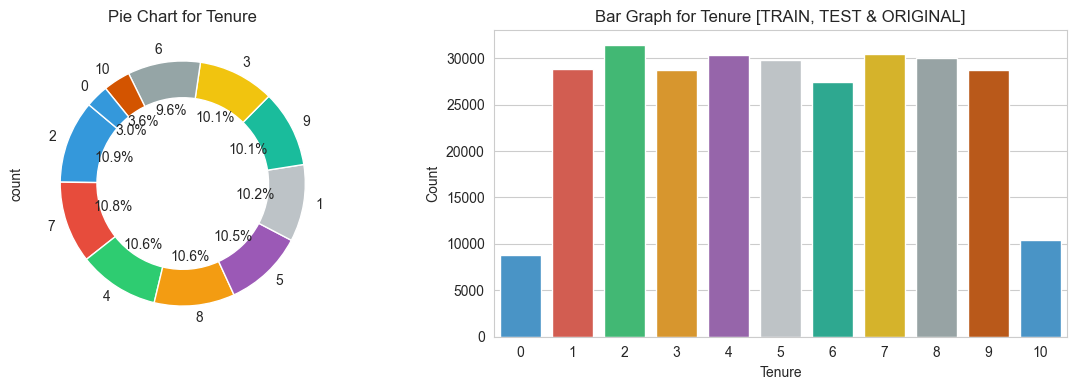
\includegraphics{EDA_Classification_files/figure-pdf/cell-15-output-3.png}

}

\end{figure}

\begin{figure}[H]

{\centering 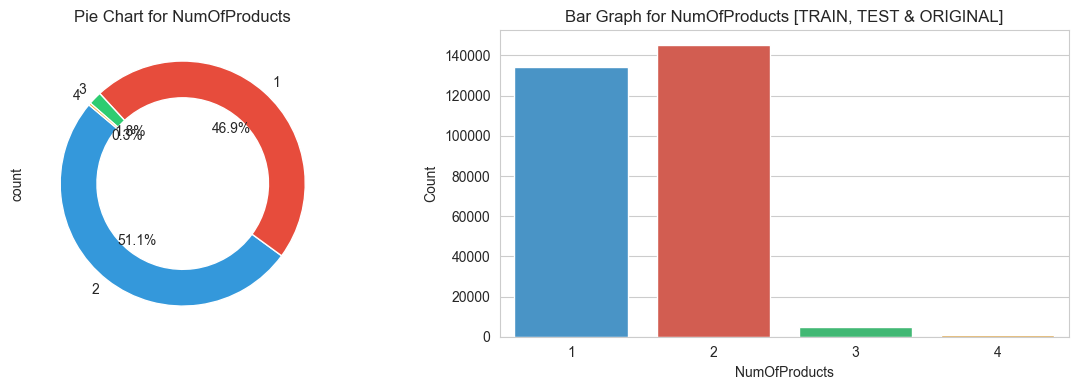
\includegraphics{EDA_Classification_files/figure-pdf/cell-15-output-4.png}

}

\end{figure}

\begin{figure}[H]

{\centering 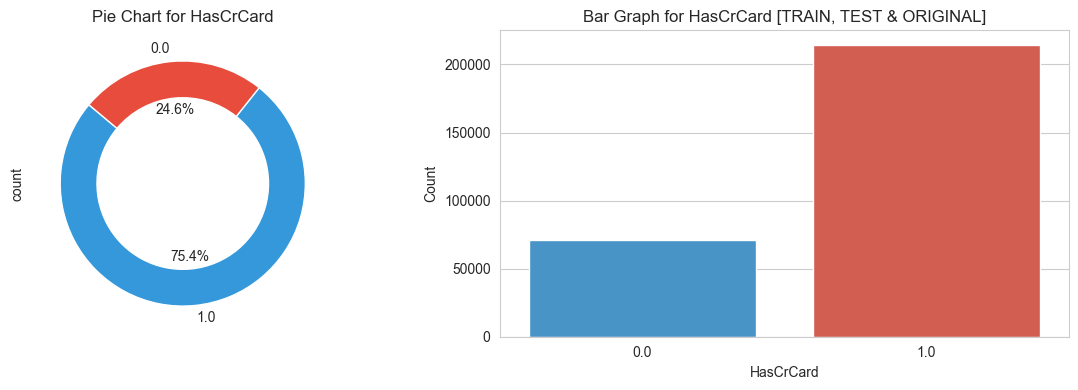
\includegraphics{EDA_Classification_files/figure-pdf/cell-15-output-5.png}

}

\end{figure}

\begin{figure}[H]

{\centering 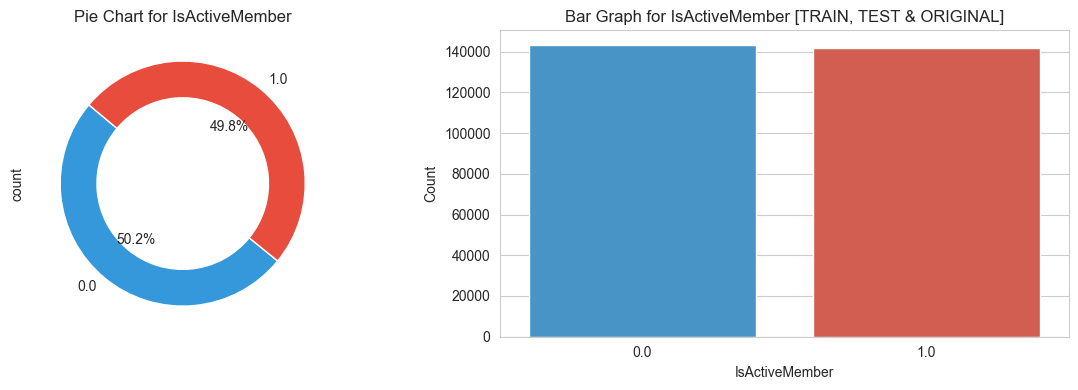
\includegraphics{EDA_Classification_files/figure-pdf/cell-15-output-6.png}

}

\end{figure}

\hypertarget{section-7}{%
\subsection{}\label{section-7}}

2

3.3 Target features

\begin{Shaded}
\begin{Highlighting}[]
\CommentTok{\# Analysis of TARGET feature}

\CommentTok{\# Define a custom color palette for categorical features}
\NormalTok{target\_palette }\OperatorTok{=}\NormalTok{ [}\StringTok{\textquotesingle{}\#3498db\textquotesingle{}}\NormalTok{, }\StringTok{\textquotesingle{}\#e74c3c\textquotesingle{}}\NormalTok{]}

\NormalTok{fig, axes }\OperatorTok{=}\NormalTok{ plt.subplots(}\DecValTok{1}\NormalTok{, }\DecValTok{2}\NormalTok{, figsize }\OperatorTok{=}\NormalTok{ (}\DecValTok{12}\NormalTok{, }\DecValTok{4}\NormalTok{))}

\CommentTok{\# Pie Chart}
\NormalTok{plt.subplot(}\DecValTok{1}\NormalTok{,}\DecValTok{2}\NormalTok{,}\DecValTok{1}\NormalTok{)}
\NormalTok{train\_data[target\_variable].value\_counts().plot.pie(}
\NormalTok{    autopct}\OperatorTok{=}\StringTok{\textquotesingle{}}\SpecialCharTok{\%1.1f\%\%}\StringTok{\textquotesingle{}}\NormalTok{, colors}\OperatorTok{=}\NormalTok{ target\_palette, }
\NormalTok{    wedgeprops}\OperatorTok{=}\BuiltInTok{dict}\NormalTok{(width}\OperatorTok{=}\FloatTok{0.3}\NormalTok{), startangle}\OperatorTok{=}\DecValTok{140}
\NormalTok{)}
\NormalTok{plt.title(}\SpecialStringTok{f"Pie Chart for Target Feature \textquotesingle{}Exited\textquotesingle{}"}\NormalTok{)}

\CommentTok{\# Bar Graph}
\NormalTok{plt.subplot(}\DecValTok{1}\NormalTok{,}\DecValTok{2}\NormalTok{,}\DecValTok{2}\NormalTok{)}
\NormalTok{sns.countplot(data}\OperatorTok{=}\NormalTok{pd.concat([}
\NormalTok{    train\_data, orignal\_data.dropna()}
\NormalTok{]),}
\NormalTok{              x}\OperatorTok{=}\NormalTok{target\_variable, palette}\OperatorTok{=}\NormalTok{target\_palette)}
\NormalTok{plt.xlabel(variable)}
\NormalTok{plt.ylabel(}\StringTok{\textquotesingle{}Count\textquotesingle{}}\NormalTok{)}
\NormalTok{plt.title(}\SpecialStringTok{f"Bar Graph for Target Feature \textquotesingle{}Exited\textquotesingle{}"}\NormalTok{)}

\CommentTok{\# adjust spacing}
\NormalTok{plt.tight\_layout()}

\CommentTok{\# show}
\NormalTok{plt.show()}
\end{Highlighting}
\end{Shaded}

\begin{figure}[H]

{\centering 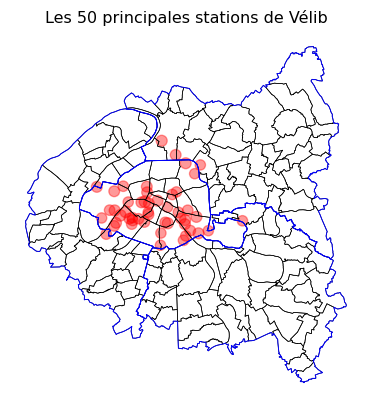
\includegraphics{EDA_Classification_files/figure-pdf/cell-16-output-1.png}

}

\end{figure}

\hypertarget{section-8}{%
\subsection{}\label{section-8}}

2

3.4 Bivariate Analysis

\begin{Shaded}
\begin{Highlighting}[]
\NormalTok{variables }\OperatorTok{=}\NormalTok{ [col }\ControlFlowTok{for}\NormalTok{ col }\KeywordTok{in}\NormalTok{ train\_data.columns }\ControlFlowTok{if}\NormalTok{ col }\KeywordTok{in}\NormalTok{ numerical\_variables]}

\NormalTok{cat\_variables\_train }\OperatorTok{=}\NormalTok{ [}\StringTok{\textquotesingle{}NumOfProducts\textquotesingle{}}\NormalTok{, }\StringTok{\textquotesingle{}HasCrCard\textquotesingle{}}\NormalTok{, }\StringTok{\textquotesingle{}IsActiveMember\textquotesingle{}}\NormalTok{, }\StringTok{\textquotesingle{}Tenure\textquotesingle{}}\NormalTok{, }\StringTok{\textquotesingle{}Exited\textquotesingle{}}\NormalTok{]}
\NormalTok{cat\_variables\_test }\OperatorTok{=}\NormalTok{ [}\StringTok{\textquotesingle{}NumOfProducts\textquotesingle{}}\NormalTok{, }\StringTok{\textquotesingle{}HasCrCard\textquotesingle{}}\NormalTok{, }\StringTok{\textquotesingle{}IsActiveMember\textquotesingle{}}\NormalTok{, }\StringTok{\textquotesingle{}Tenure\textquotesingle{}}\NormalTok{]}

\CommentTok{\# Adding variables to the existing list}
\NormalTok{train\_variables }\OperatorTok{=}\NormalTok{ variables }\OperatorTok{+}\NormalTok{ cat\_variables\_train}
\NormalTok{test\_variables }\OperatorTok{=}\NormalTok{ variables }\OperatorTok{+}\NormalTok{ cat\_variables\_test}

\CommentTok{\# Calculate correlation matrices for train\_data and test\_data}
\NormalTok{corr\_train }\OperatorTok{=}\NormalTok{ train\_data[train\_variables].corr()}
\NormalTok{corr\_test }\OperatorTok{=}\NormalTok{ test\_data[test\_variables].corr()}

\CommentTok{\# Create masks for the upper triangle}
\NormalTok{mask\_train }\OperatorTok{=}\NormalTok{ np.triu(np.ones\_like(corr\_train, dtype}\OperatorTok{=}\BuiltInTok{bool}\NormalTok{))}
\NormalTok{mask\_test }\OperatorTok{=}\NormalTok{ np.triu(np.ones\_like(corr\_test, dtype}\OperatorTok{=}\BuiltInTok{bool}\NormalTok{))}

\CommentTok{\# Set the text size and rotation}
\NormalTok{annot\_kws }\OperatorTok{=}\NormalTok{ \{}\StringTok{"size"}\NormalTok{: }\DecValTok{8}\NormalTok{, }\StringTok{"rotation"}\NormalTok{: }\DecValTok{45}\NormalTok{\}}

\CommentTok{\# Generate heatmaps for train\_data}
\NormalTok{plt.figure(figsize}\OperatorTok{=}\NormalTok{(}\DecValTok{15}\NormalTok{, }\DecValTok{5}\NormalTok{))}
\NormalTok{plt.subplot(}\DecValTok{1}\NormalTok{, }\DecValTok{2}\NormalTok{, }\DecValTok{1}\NormalTok{)}
\NormalTok{ax\_train }\OperatorTok{=}\NormalTok{ sns.heatmap(corr\_train, mask}\OperatorTok{=}\NormalTok{mask\_train, cmap}\OperatorTok{=}\StringTok{\textquotesingle{}viridis\textquotesingle{}}\NormalTok{, annot}\OperatorTok{=}\VariableTok{True}\NormalTok{,}
\NormalTok{                      square}\OperatorTok{=}\VariableTok{True}\NormalTok{, linewidths}\OperatorTok{=}\FloatTok{.5}\NormalTok{, xticklabels}\OperatorTok{=}\DecValTok{1}\NormalTok{, yticklabels}\OperatorTok{=}\DecValTok{1}\NormalTok{, annot\_kws}\OperatorTok{=}\NormalTok{annot\_kws)}
\NormalTok{plt.title(}\StringTok{\textquotesingle{}Correlation Heatmap {-} Train Data\textquotesingle{}}\NormalTok{)}

\CommentTok{\# Generate heatmaps for test\_data}
\NormalTok{plt.subplot(}\DecValTok{1}\NormalTok{, }\DecValTok{2}\NormalTok{, }\DecValTok{2}\NormalTok{)}
\NormalTok{ax\_test }\OperatorTok{=}\NormalTok{ sns.heatmap(corr\_test, mask}\OperatorTok{=}\NormalTok{mask\_test, cmap}\OperatorTok{=}\StringTok{\textquotesingle{}viridis\textquotesingle{}}\NormalTok{, annot}\OperatorTok{=}\VariableTok{True}\NormalTok{,}
\NormalTok{                     square}\OperatorTok{=}\VariableTok{True}\NormalTok{, linewidths}\OperatorTok{=}\FloatTok{.5}\NormalTok{, xticklabels}\OperatorTok{=}\DecValTok{1}\NormalTok{, yticklabels}\OperatorTok{=}\DecValTok{1}\NormalTok{, annot\_kws}\OperatorTok{=}\NormalTok{annot\_kws)}
\NormalTok{plt.title(}\StringTok{\textquotesingle{}Correlation Heatmap {-} Test Data\textquotesingle{}}\NormalTok{)}

\CommentTok{\# Adjust layout}
\NormalTok{plt.tight\_layout()}

\CommentTok{\# Show the plots}
\NormalTok{plt.show()}
\end{Highlighting}
\end{Shaded}

\begin{figure}[H]

{\centering 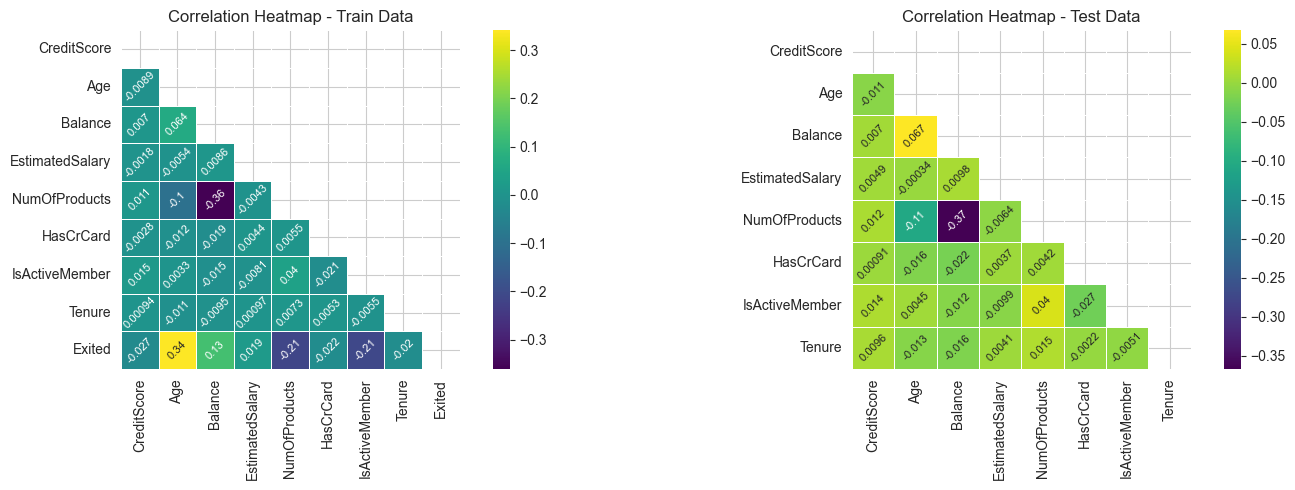
\includegraphics{EDA_Classification_files/figure-pdf/cell-17-output-1.png}

}

\end{figure}



\end{document}
